\documentclass{article}

\usepackage{graphicx}
\usepackage{tikz}
\usepackage{tikzsymbols}
\usetikzlibrary{calc,patterns,shapes.geometric}
\pagestyle{empty}
\usepackage[margin=0pt]{geometry}
\geometry{papersize={14in,12in}}

\def\centerarc[#1](#2)(#3:#4:#5){\draw[#1] ($(#2)+({#5*cos(#3)},{#5*sin(#3)})$) arc (#3:#4:#5);}

\begin{document}
	\begin{figure}
		\centering
		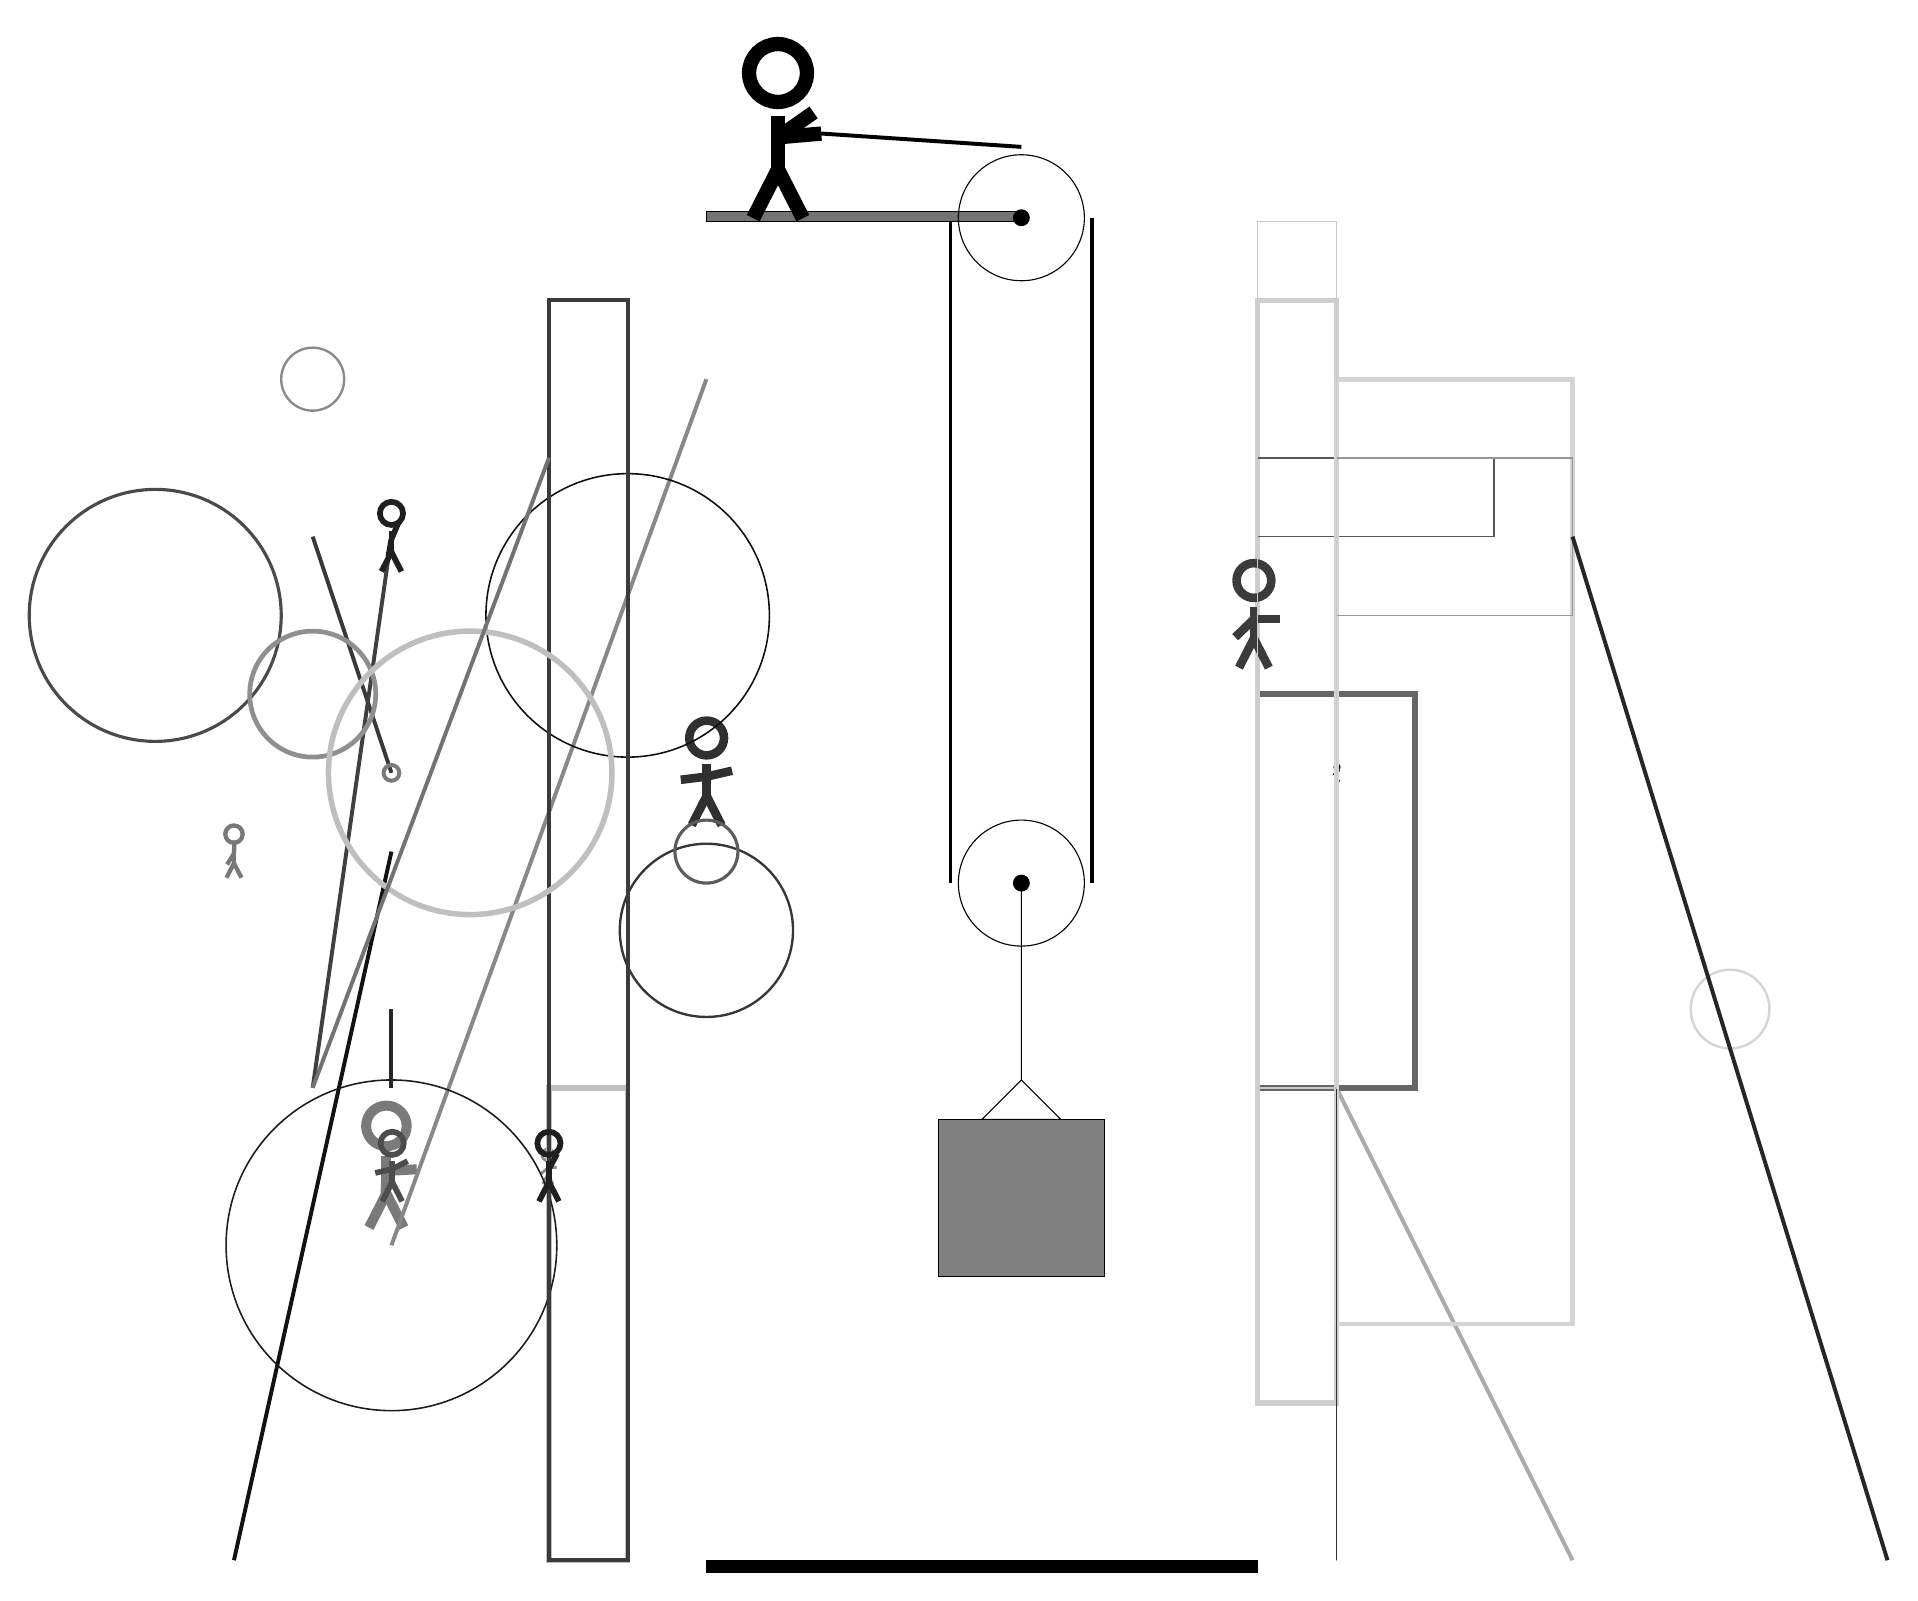
\begin{tikzpicture}
			%%%%% START %%%%%
			
			\draw[fill=black!55] (-2, 14) rectangle (2, 14.125);
			
			\draw (2, 5.6) circle (0.8);
			\draw[fill=black] (2, 5.6) circle (0.1);
			
			\draw (2, 14.05) circle (0.8);
			\draw[fill=black] (2, 14.05) circle (0.1);
			
			\draw [line width=0.3mm, color=black!79](-2, 5) circle (1.1);
			
			\draw[line width=0.5mm, color=black!78](-6, 7) -- (-7, 10);
			\draw[line width=0.5mm, color=black!75](-7, 3) -- (-6, 10);
			\node[line width=0.5mm, color=black!52] at (-6, 2) {\Strichmaxerl[7][88][3]};
			\draw[line width=0.5mm, color=black!47](-6, 1) -- (-2, 12);
			
			\draw[line width=0.5mm, color=black!93](-6, 6) -- (-8, -3);
			
			\draw[line width=0.5mm, color=black!33](9, -3) -- (6, 3);
			\draw [line width=0.3mm, color=black!46](-7, 12) circle (0.4);
			\draw[line width=0.7mm, color=black!60] (5, 8) rectangle (7, 3);
			\draw [line width=0.5mm, color=black!52](-6, 7) circle (0.1);
			\node[line width=0.3mm, color=black!70] at (-6, 2) {\Strichmaxerl[4][13][27]};
			\node[line width=0.7mm, color=black!88] at (-6, 10) {\Strichmaxerl[4][80][67]};
			\draw [line width=0.4mm, color=black!71](-9, 9) circle (1.6);
			
			\node[line width=0.2mm, color=black!81] at (-2, 7) {\Strichmaxerl[6][7][13]};
			\draw [line width=0.2mm, color=black!94](-3, 9) circle (1.8);
			\draw[line width=0.7mm, color=black!19] (5, 13) rectangle (6, -1);
			\node[line width=0.7mm, color=black!45] at (-4, 2) {\Strichmaxerl[2][41][3]};
			\draw [line width=0.3mm, color=black!17](11, 4) circle (0.5);
			\draw[line width=0.2mm, color=black!66] (5, 10) rectangle (8, 11);
			
			\draw[line width=0.7mm, color=black!25] (-4, -3) rectangle (-3, 3);
			\draw[line width=0.5mm, color=black!95](-3, 4) -- (-3, 1);
			\draw [line width=0.2mm, color=black!89](-6, 1) circle (2.1);
			\draw[line width=0.5mm, color=black!85](-6, 3) -- (-6, 4);
			\draw[line width=0.5mm, color=black!77] (-3, -3) rectangle (-4, 13);
			\node[line width=0.5mm, color=black!77] at (5, 9) {\Strichmaxerl[6][44][0]};
			\node[line width=0.6mm, color=black!95] at (6, 7) {\Strichmaxerl[1][12][53]};
			
			\draw [line width=0.6mm, color=black!44](-7, 8) circle (0.8);
			\draw [line width=0.7mm, color=black!25](-5, 7) circle (1.8);
			\draw [line width=0.4mm, color=black!64](-2, 6) circle (0.4);
			\draw[line width=0.6mm, color=black!17] (6, 0) rectangle (9, 12);
			\draw[line width=0.2mm, color=black!41] (6, 11) rectangle (9, 9);
			
			\draw[line width=0.5mm, color=black!55](-7, 3) -- (-4, 11);
			\node[line width=0.3mm, color=black!88] at (-4, 2) {\Strichmaxerl[4][89][62]};
			
			\draw[line width=0.2mm, color=black!82] (6, 12) rectangle (6, -3);
			
			\node[line width=0.5mm, color=black!53] at (-8, 6) {\Strichmaxerl[3][58][88]};
			\draw[line width=0.5mm, color=black!85](9, 10) -- (13, -3);
			
			\draw[line width=0.2mm, color=black!21] (5, 3) rectangle (6, 14);
			
			\draw (2, 5.6) -- (2, 3.1) -- (1.5, 2.6) -- (2.5, 2.6) -- (2, 3.1);
			\draw[fill=black!50] (0.95, 2.6) rectangle (3.05, 0.6);
			
			\draw[line width=0.5mm] (1.1, 14) -- (1.1, 5.6);
			\centerarc[line width=0.5mm](2, 5.6)(180:360:0.9);
			\draw[line width=0.5mm](2.9, 5.6) -- (2.9, 14.05);
			\centerarc[line width=0.5mm](2, 14.05)(0:90:0.9);
			\draw[line width=0.5mm](2, 14.95) -- (-1, 15.15);
			
			\node at (-1, 15.15) {\Strichmaxerl[10][-175][35]};
			
			\draw[fill=black] (-2, -3) rectangle (5, -3.15);
			
			%%%%% END %%%%%
		\end{tikzpicture}
	\end{figure}	
\end{document}